PolarFarmBot will be a CNC robot that will automate the agricultural process. The robot will pivot around a central pole and have a tool assembly that will moved in and out along the arm of the robot.
PolarFarmBot will plant seeds, water plants, measure soil moisture levels, calculate soil pH levels, and remove weeds.
The robot will connect back to a computer that will have a web interface for users to interact with the robot. From this interface a user will be able to layout a plot, monitor overall plant growth and soil conditions, and see whether or not the plants are ready for harvesting.
To go along with the web interface, there will be a companion application developed for android. This app will have all the same functionality as the web app just on a mobile platform.
PolarFarmBot will have multiple cameras attached to it to allow monitoring progress remotely.


\begin{figure}[h!]
    \centering
    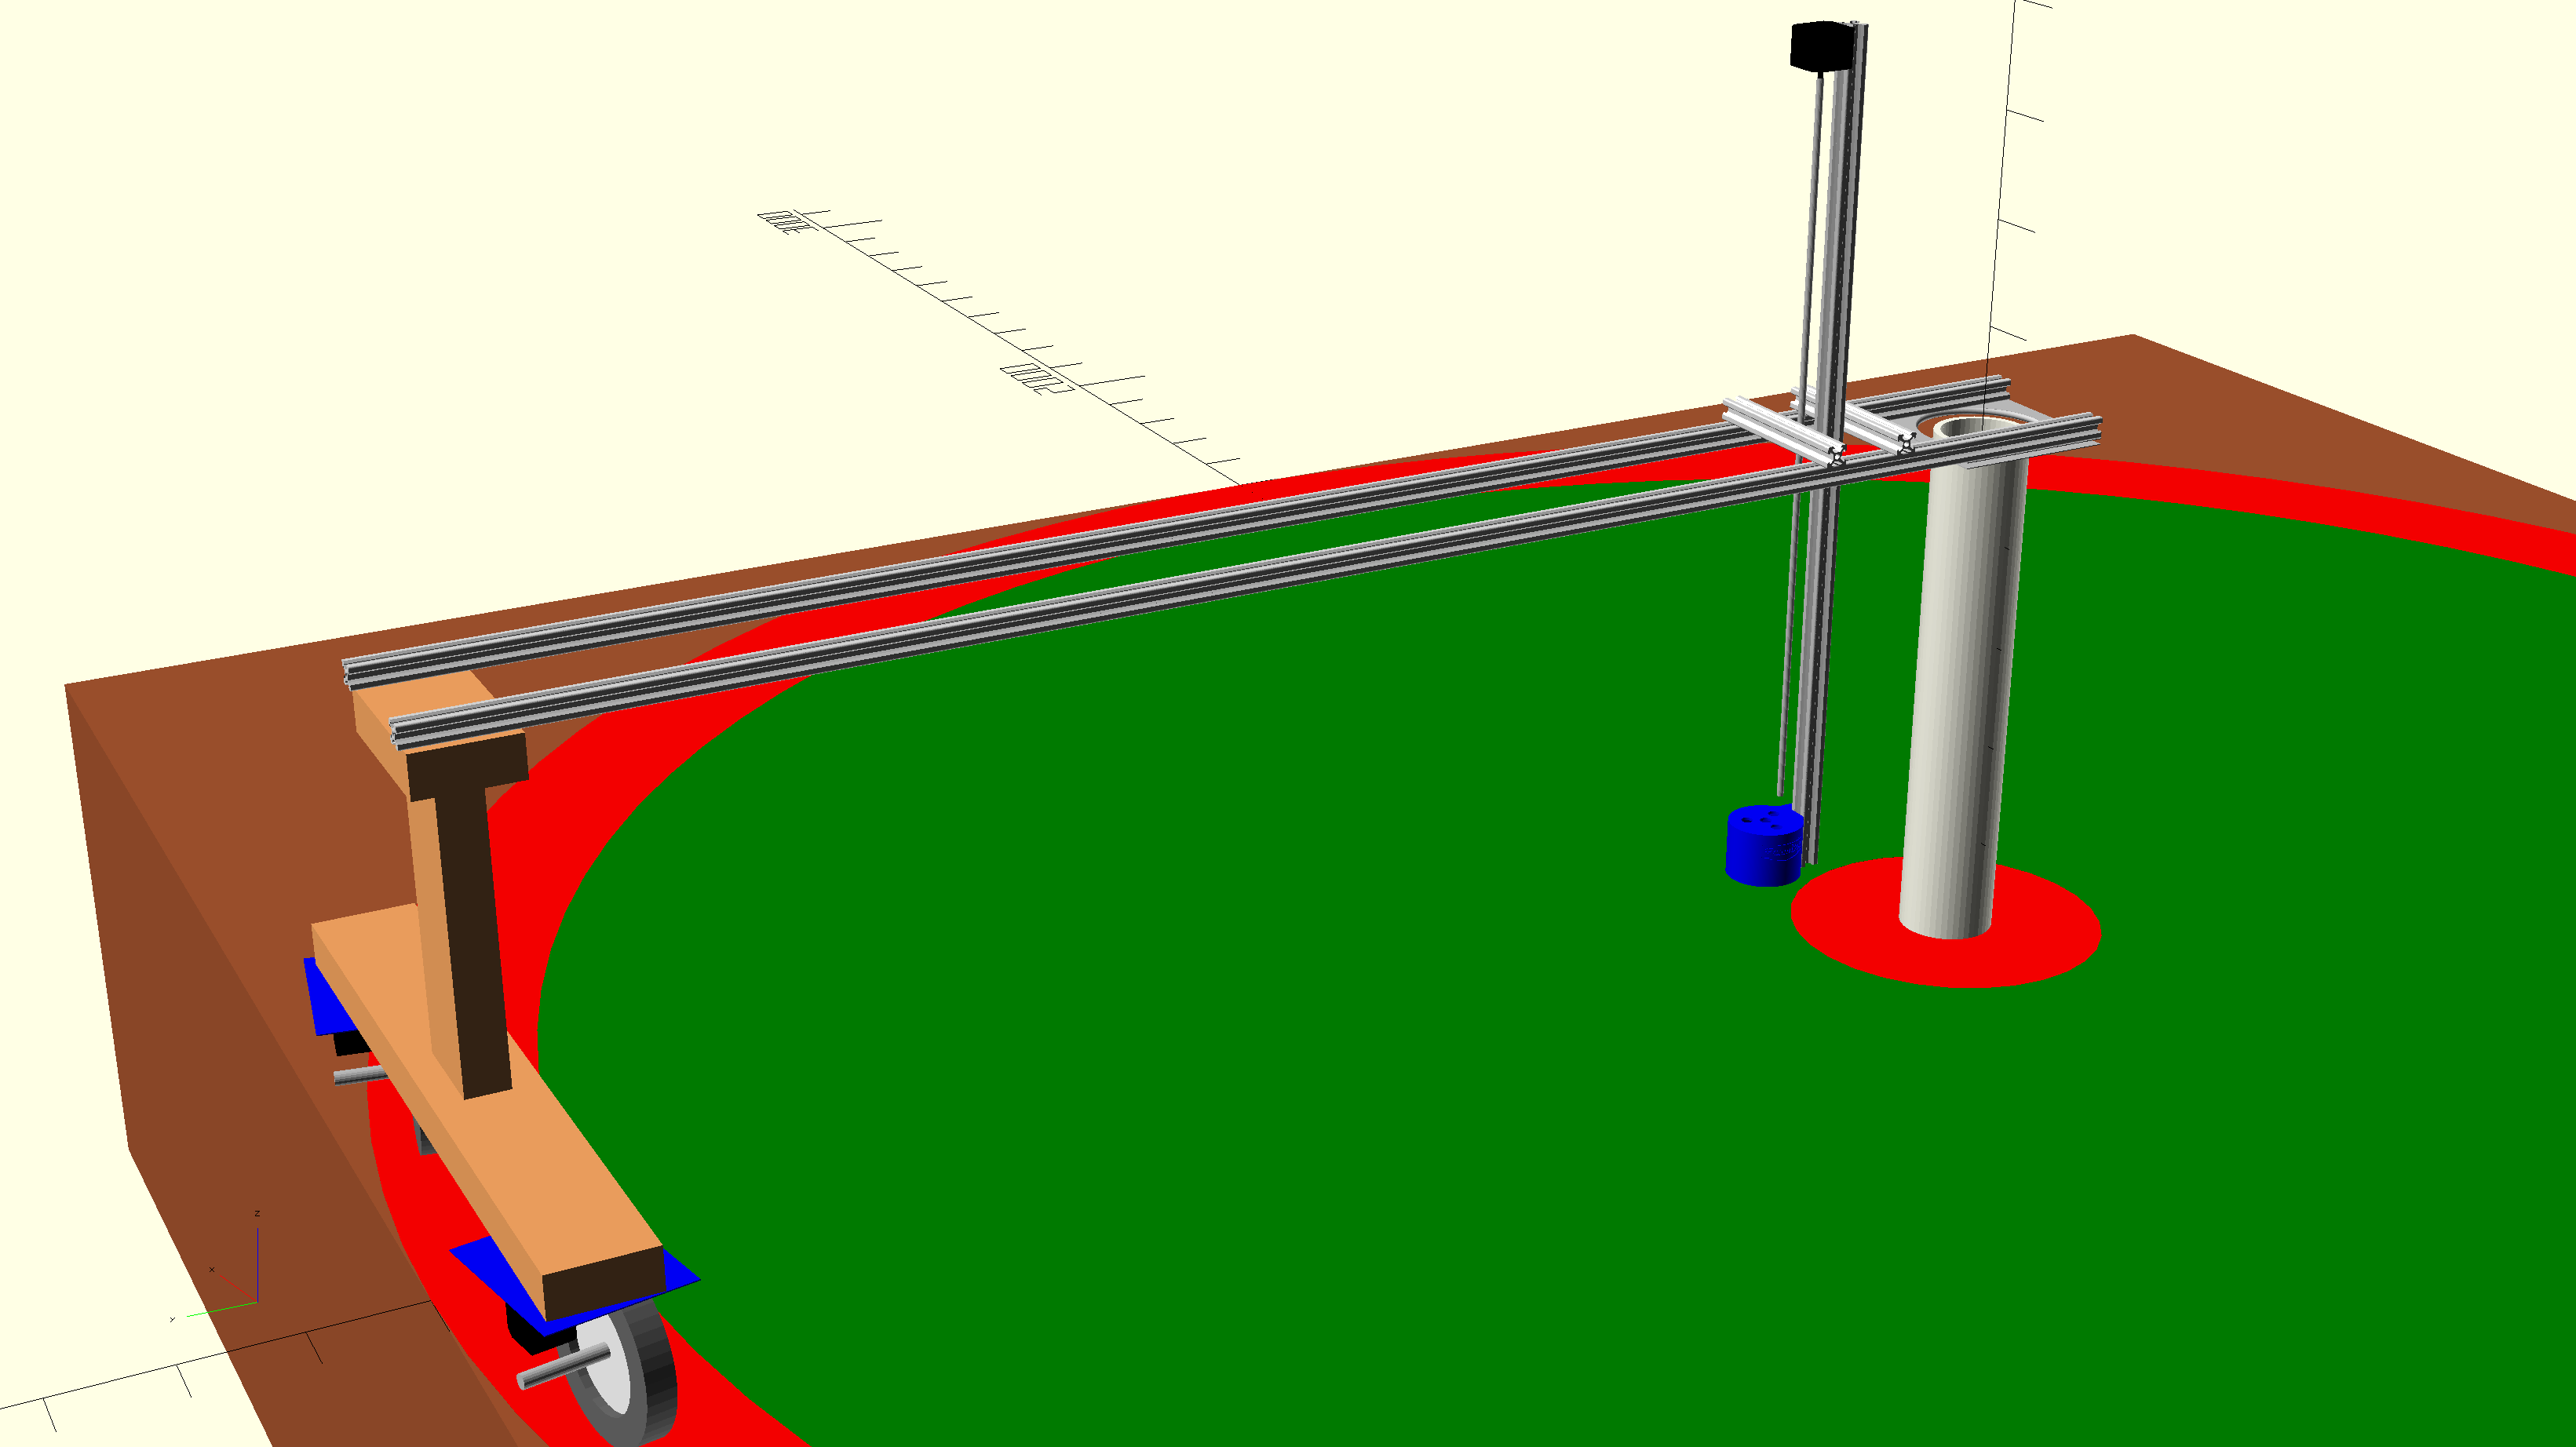
\includegraphics[width=0.75\textwidth]{images/arm-closeup}
    \caption{Deatailed view of mock-up arm design}
\end{figure}